\documentclass[a4paper]{refart}

\usepackage{url}
\usepackage{graphicx}
\usepackage{float}

\title{Leap VR Castle Defense\\User Guide}
\author{Valerie Gadjali\\
	Timothy Tong\\
	Alexandre Wimmers\\
	Mario Yepez
}
\date{Last Updated: May 27, 2015}

\begin{document}

\maketitle

\tableofcontents

\newpage

\section{Introduction}

This project was created using the following versions. Previous versions of runtime environments are outdated and will not suffice. Updates will be required.

\begin{itemize}
	\item Unity 5.0.1f1
	\item Oculus Runtime 0.6.0.0-beta
	\item Leap Motion 2.2.5
	\item Leap Motion Core Assets 2.2.4
\end{itemize}

\section{Software Requirements}

\begin{enumerate}
	\item Oculus Runtime.\\ \url{https://developer.oculus.com/downloads/}.
	\item Leap Motion Setup.\\ \url{https://www.leapmotion.com/setup}.
	\item Unity 5 engine.\\ \url{https://unity3d.com/get-unity/download}.
\end{enumerate}

\section{Game Installation}

No installation required. The Unity system behaves very similarly to Java. The Unity runtime environment acts like the Java Virtual Machine so installation of the game engine will suffice. 

\textbf{***Critical:} Development of game was perform strictly in Windows 7 and not extensively tested on OSX or Linux.

\pagebreak

\section{Gameplay}

\begin{enumerate}
	\item First, make sure that both the Oculus Rift and the Leap Motion devices are on and connected to your computer.
	\item To run the game, start by executing:\\
		 \texttt{LeapVRCastleDefense\_DirectToRift.exe}\footnote{On OSX, DirectToRift.exe is not supported, to run the game mirror your display to the Rift, execute \texttt{LeapVRCastleDefense.app}, and position the window correctly.}
	\item Put on the Oculus Rift.
	\item A game menu will appear. Move your hands in front of the Leap Motion device and press the \texttt{Start} button.
	\item Enemies will begin spawning. The enemies will constantly run towards the castle and attempt to damage it. 
	\item You, as the player, must defend your castle. To defend your castle, you can use your hands to pick up the enemies and toss them into the air. When they fall and hit the ground, they will receive damage. 
	\item Enemies can also spawn from any direction so you will need to rotate your head and/or body to constantly look around.
	\item When all enemies on the current level are defeated, a countdown is shown at the top. This is the countdown until the next wave of enemies spawn. 
	\item The game continues until player runs out of health.
	\item The goal is to get as many points as possible before running out of health.
\end{enumerate}

\newpage

\section{Further Development}

\subsection{Extending from the Current Leap VR Castle Defense}

\begin{figure}[h]
	\centering
	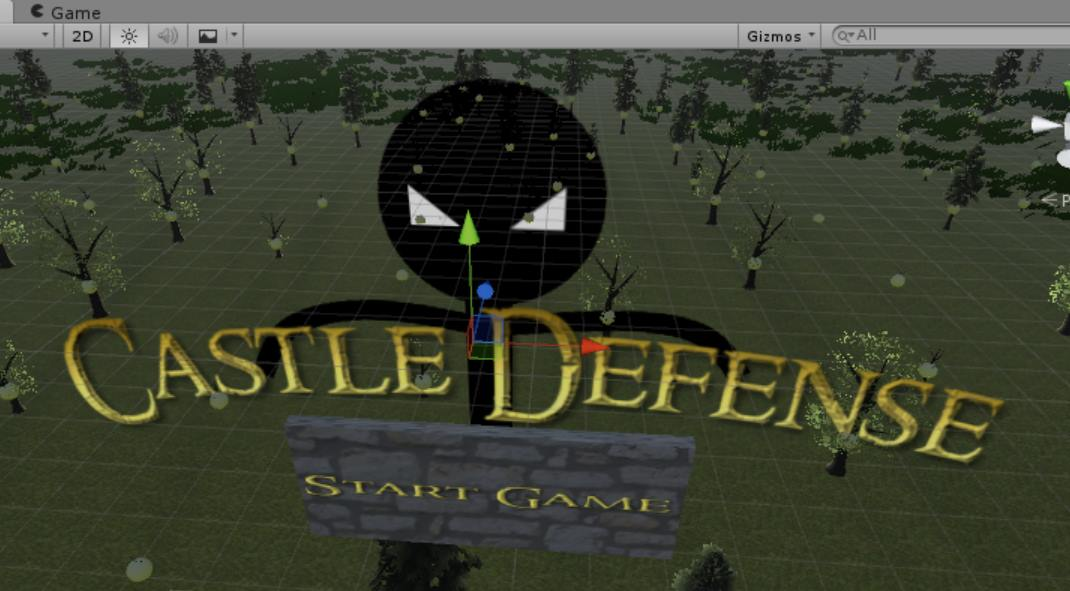
\includegraphics[width=\textwidth]{scene.jpg}
\end{figure}


\textbf{*** This guide is written with the assumption that the developer is familiar with the Unity game engine.}

\textbf{*** All Unity game scripts are written in C\#.}

\subsubsection{Getting the Codebase}

\begin{enumerate}
	\item Clone the Bitbucket repository:\\ \url{git@bitbucket.org:ecs193/project.git}
	\item From here on, the $<$ROOT$>$ directory will be referred to where the project directory is. If you pulled directly from the repository, it will be in directory \texttt{project-unity5}.
\end{enumerate}

\subsubsection{Load the Project}

Directory: \texttt{$<$ROOT$>$/Scenes/}

\begin{enumerate}
	\item Open \texttt{main.unity} in the Unity game engine.
\end{enumerate}

\subsubsection{Edit the Map}

\begin{enumerate}
	\item Using Unity's terrain tools, modify the map.
	\item To add new entities, drag and drop Prefabs from the Project windows into the Scene window or the Hierarchy window.
\end{enumerate}

\subsubsection{Modify Enemies}

Directory: \texttt{$<$ROOT$>$/Assets/Custom/Prefabs/Enemies/}

\begin{enumerate}
	\item Enemy entities are notated by the \texttt{.prefab} extension in this folder.
	\item To change the model, modify the renderer component.
	\item To modify the enemy behavior, modify any of the scripts attached to the enemies.
	\begin{itemize}
		\item EnemyAttack.cs (Enemy script to attack player)
		\item EnemyHealth.cs (Enemy script to handle enemy health)
		\item EnemyMovement.cs (Enemy script to handle movement)
	\end{itemize}
\end{enumerate}

\subsubsection{Modify Game Behavior}

Directory: \texttt{$<$ROOT$>$/Assets/Custom/Prefabs/Managers/}

\begin{enumerate}
	\item Modify the EnemyManager.prefab to change Enemy spawn types.
	\item Modify the GameManager.prefab to change Enemy spawning behavior and Day Night Cycle.
\end{enumerate}

The GameManager prefab coordinates with all EnemyManagers and controls the waves in which the enemies come. Each respective EnemyManager only focuses on spawning the enemy type it is in charge of.

\subsubsection{Modify Pinching Behavior}

Directory: \texttt{$<$ROOT$>$/Assets/LeapMotion/Scripts/Utils/}

\begin{enumerate}
	\item Modify script \texttt{MagneticPinch.cs}.
	\item Modify the function: \texttt{OnPinch(...)}
\end{enumerate}

In function, \texttt{OnPinch(...)}, array of Collider objects is array of game entities that are within pinching distance. The following for-loop is to select the closest entity among those that are within pinching distance. This allows the hand to grab only one object at a time.
\end{document}